\documentclass[10pt,a4paper]{article}
\usepackage[utf8]{inputenc}
\usepackage[croatian]{babel}
\usepackage{amsmath}
\usepackage{amsfonts}
\usepackage{amssymb}
\usepackage{graphicx}
\usepackage[left=2cm,right=2cm,top=2cm,bottom=2cm]{geometry}
\author{Luka Skukan}
\title{Ra\v{c}unalna Grafika\\Samostalna Laboratorijska Vje\v{z}ba\\Pong}
\date{}
\begin{document}
\maketitle

\section{Opis igre Pong}

Pong je jednostavna dvodimenzionalna igra. Postoje dva igra\v{c}a (ljudi ili ra\v{c}unalni programi), koji upravljaju dvama ``reketima'' koji se nalaze na lijevom, odnosno desnom, kraju ekrana, te se mogu kretati samo vertikalno (gore ili dolje). Izme\dj{}u dva igra\v{c}a giba se loptica. Loptica se odbija od gornjeg i donjeg ruba ekrana, kao i od igra\v{c}kih reketa. Ukoliko loptica pogodi rub ekrana iza jednog od reketa, igra\v{c} na suprotnoj strani dobiva bod.

\begin{figure}[h]
	\center
	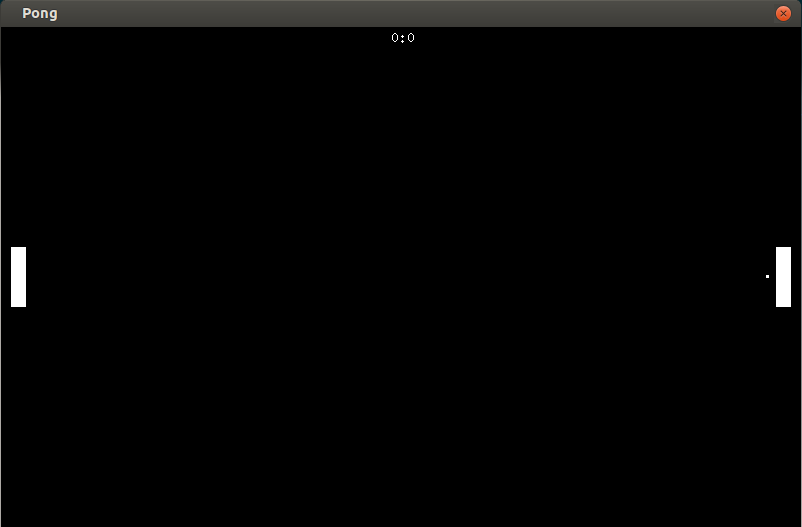
\includegraphics[scale=0.5]{pong}
	\caption{Igra Pong}
\end{figure}

\section{Implementacija igre}

Potrebno je implementirati jednostavnu verziju igre Pong, gdje jedan igra\v{c} igra protiv ra\v{c}unala. Potrebno je napraviti animiranje objekata (reketa i loptice) uz obradu pona\v{s}anja pri sudaru, prikaz rezultata, kao i osmisliti i implementirati pona\v{s}anje drugog igra\v{c}a, kojim upravlja ra\v{c}unalo.

Pri sudaru loptice i reketa, loptica se mora odbiti pod kutem, u ovisnosti o tome u koji dio reketa udara. Ukoliko udara u sredi\v{s}te reketa, odbija se ravno prema suprotnoj strani. \v{S}to je udarac bli\v{z}e rubu reketa, loptica se odbija vi\v{s}e u stranu, u tom smjeru. Odabir kuta je proizvoljan.

Potrebno je izra\v{c}unati, prikazati i osvje\v{z}iti rezultat pri svakom sudaru loptice sa zidom iza jednog od reketa. Kada igra\v{c} postigne poen, loptica se vra\'{c}a u centralni polo\v{z}aj te kre\'{c}e prema igra\v{c}u koji je taj poen postigao.

\subsection{Detekcija sudara}

Kako bi se pravilno implementiralo odbijanje loptice, potrebno je vr\v{s}iti detekciju sudara. Budu\'{c}i da se radi o krugu u dvije dimenzije, detekcija je jednostavna:

\begin{itemize}
	\item Loptica se sudara sa zidom ukoliko bi u kretanju trenutnom brzinom njezin rub (polo\v{z}aj centra plus njen radijus) dotaknuo ili presjekao polo\v{z}aj zida.
	\item Loptica se sudara sa reketom ukoliko vrijedi isto, ali loptica je tako\dj{}er vertikalno u kontaktu sa reketom (reket ne pokriva cijelu vertikalnu udaljenost ekrana).
\end{itemize}

\subsection{Implementacija umjetne inteligencije igra\v{c}a}

Protivni\v{c}kim igra\v{c}em mora upravljati ra\v{c}unalo. Potrebno je implementirati sustav koji odlu\v{c}uje koji pokret ra\v{c}unalo vr\v{s}i u svakom koraku. Algoritam mo\v{z}e biti vrlo jednostavan -- primjerice centar reketa mora pratiti poziciju loptice.

\end{document}
